\documentclass[a4paper,12pt]{article} % тип документа

% Поля страниц
\usepackage[left=2.5cm,right=2.5cm,
    top=2cm,bottom=2cm,bindingoffset=0cm]{geometry}
    
%Пакет дял таблиц   
\usepackage{multirow} 
    
%Отступ после заголовка    
\usepackage{indentfirst}


% Рисунки
\usepackage{floatrow,graphicx,calc}
\usepackage{wrapfig}

%%% Работа с картинками
\usepackage{graphicx}  % Для вставки рисунков
\graphicspath{{images/}}  % папки с картинками
\setlength\fboxsep{3pt} % Отступ рамки \fbox{} от рисунка
\setlength\fboxrule{1pt} % Толщина линий рамки \fbox{}
\usepackage{wrapfig} % Обтекание рисунков и таблиц текстом

% Создаём новый разделитель
\DeclareFloatSeparators{mysep}{\hspace{1cm}}

% Ссылки?
\usepackage{hyperref}
\usepackage[rgb]{xcolor}
\hypersetup{				% Гиперссылки
    colorlinks=true,       	% false: ссылки в рамках
	urlcolor=blue          % на URL
}


%  Русский язык
\usepackage[T2A]{fontenc}			% кодировка
\usepackage[utf8]{inputenc}			% кодировка исходного текста
\usepackage[english,russian]{babel}	% локализация и переносы

% Математика
\usepackage{amsmath,amsfonts,amssymb,amsthm,mathtools}

%%% Дополнительная работа с математикой
\usepackage{amsmath,amsfonts,amssymb,amsthm,mathtools} % AMS
\usepackage{icomma} % "Умная" запятая: $0,2$ --- число, $0, 2$ --- перечисление

% Что-то 
\usepackage{wasysym}


\begin{document}
\begin{center}
	\footnotesize{ФЕДЕРАЛЬНОЕ ГОСУДАРСТВЕННОЕ АВТОНОМНОЕ ОБРАЗОВАТЕЛЬНОЕ 			УЧРЕЖДЕНИЕ ВЫСШЕГО ОБРАЗОВАНИЯ}\\
	\footnotesize{МОСКОВСКИЙ ФИЗИКО-ТЕХНИЧЕСКИЙ ИНСТИТУТ\\(НАЦИОНАЛЬНЫЙ 			ИССЛЕДОВАТЕЛЬСКИЙ УНИВЕРСИТЕТ)}\\
	\footnotesize{ФИЗТЕХ-ШКОЛА ФИЗИКИ И ИССЛЕДОВАНИЙ им. ЛАНДАУ\\}
	\hfill \break
	\hfill \break
	\hfill \break
	\hfill \break
\end{center}

\begin{center}   
    \hfill \break
	\hfill \break
	\hfill \break
	\hfill \break    \hfill \break
	\hfill \break
	\hfill \break
	\hfill \break
    \hfill \break
    \hfill \break
	\hfill \break
	\large{Лабораторная работа № 2.4.1\\\textbf{Определение теплоты испарения жидкости}}\\
	\begin{flushright}
		Плотникова Анастасия Александровна\\
		Группа Б02-406
	\end{flushright}
	\hfill \break
	\hfill \break
	\hfill \break
\end{center}
\hfill \break
\hfill \break
\hfill \break
\hfill \break
\hfill \break
\hfill \break
\hfill \break
\hfill \break
\hfill \break
\hfill \break
\hfill \break
\hfill \break
\hfill \break
\begin{center}
	Долгопрудный, 2025 г.
\end{center}
\thispagestyle{empty}
\newpage
	\textbf{Цель работы:}\\ 
  1) измерение давления насыщенного пара жидкости при разной температуре;\\ 
  2) вычисление по полученным данным теплоты испарения с помощью уравения Клапейрона-Клаузиуса.
	\hfill \break
	
	\textbf{В работе используются:}\\ 
  термостат TERMEX BT-po-02 ($dT = 0.03$ K),\\ 
  герметический сосуд, заполненный водой,\\ 
  отсчетный микроскоп,\\
  электронный штангенциркуль ($dh = 0.03$ мм).
	
\section*{Теоретическая справка}

\textit{Испарение} — переход вещества из жидкого в газообразное состояние 
на свободной поверхности жидкости. 

Для выхода из жидкости молекуля должны совершить работу против сил молекулярного сцепления, 
внешнего давления, для чего должны обладать достаточной кинетической энергией. Переход части 
быстрых молекул в пар сопровождается потерями энергии, следовательно, и охлаждением жидкости.

\textit{Молярная теплота испарения (парообразования)} — количество теплоты, необходимое для 
изотермического испарения одного моля жидкости при внешнем давлении, равном упругости ее насыщенных паров.
    
В настоящей работе для определения теплоты испарения применен косвенный метод, 
основанный на формуле Клапейрона-Клаузиуса:
\begin{equation}
    \label{Klap}
    \frac{dP}{dT} = \frac{L}{T(V_2 - V_1)}
\end{equation}

\noindent $P$ -- давление насыщенного пара жидкости при температуре $T$,\\ 
$T$ -- абсолютная температура жидкости и пара,\\ 
$L$ — теплота испарения жидкости,\\ 
$V_2$ -- объем пара,\\ 
$V_1$ -- объем жидкости.

\begin{table}[h]
  \centering
  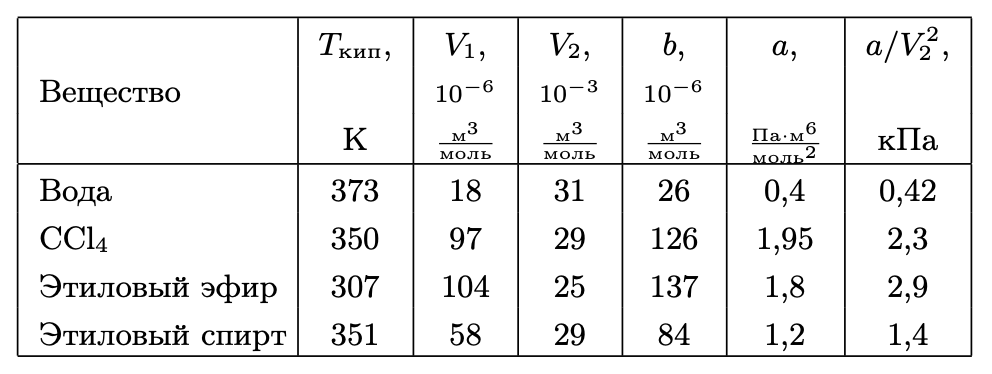
\includegraphics[scale = 0.55]{table_data.png}
  \caption{Табличные данные}
  \label{fig:table_data}
\end{table}

Найдя из опыта $dP/dT$, $T$, $V_2$ и $V_1$, можно определить $L$ путем расчета. 
Величины $L$, $V_2$ и $V_1$ в формуле (\ref{Klap}) должны относиться к одному и 
тому же количеству вещества; мы будем относить их к одному молю.

Измерения проводятся при давлениях ниже атмосферного.

Из табличных данных видно, что $V_1$ не превосходит $0.5\%$ от $V_2$. 

\medskip

Обратимся теперь к $V_2$, которое в дальнейшем будем обозначать $V$. 
Объем $V$ связан с давелнием и темературой уравнением Ван-дер-Ваальса:

\begin{equation}
    \label{Van-der}
    \left( P + \frac{a}{V^2}\right)(V - b) = RT
\end{equation}

Из рассмотрения таблицы (\ref{fig:table_data}) следует, что $b$ одного порядка с $V_1$. 
В уравнении Ван-дер-Ваальса величиной $b$ следует пренебречь. Пренебрежение членом $a/V^2$ 
по сравнению с $P$ вносит ошибку менее 3\%. 
При давлении ниже атмосферного ошибки становятся еще меньше. 

Таким образом, при давлениях ниже атмосферного уравнение Ван-дер-Ваальса для насыщенного пара 
мало отличается от уравнения Клапейрона. Положим поэтому

\begin{equation}
    \label{ideal}
    P = \frac{RT}{V}
\end{equation}

Подставляя (\ref{ideal}) в (\ref{Klap}) и разрешая уравение относительно $L$, получаем:

\begin{equation}
    \label{L}
    L = \frac{RT^2}{P}\frac{dP}{dT} = -R\frac{d(\mbox{ln }P)}{d(1/T)}
\end{equation}

Эта формула является окончательной.

\section*{Экспериментальная установка}

Схема установки изображена на рисунке (\ref{fig:drawing2}). 

\begin{figure}[h]
  \centering
  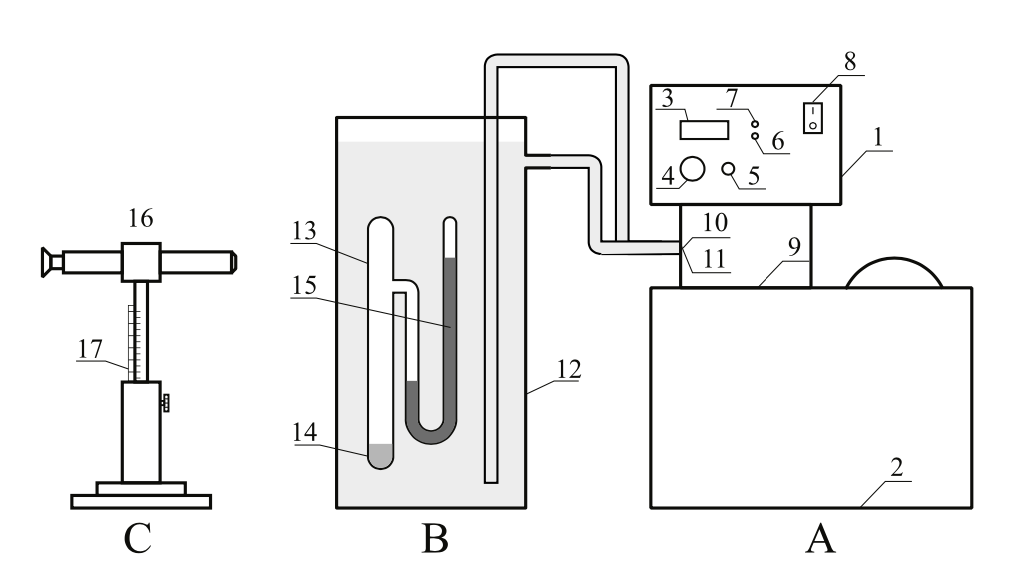
\includegraphics[scale = 0.5]{drawing2.png}
  \caption{Схема установки для определения теплоты испарения}
  \label{fig:drawing2}
\end{figure}

\noindent 12. Емкость, заполненная водой. \\
13. Запаянный прибор с исследуемой жидкостью (14). 
Перед заполнением исследуемой жидкости воздух из запаянного прибора был удалён, 
так что над жидкостью находится только её насыщенный пар. \\
14. Исследуемая жидкость.\\
15. Ртутный манометр, соединённый с ёмкостью (13). \\
16. Отсчётного микроскопа, настраиваемого последовательно на нижний и верхний 
уровни столбика ртути манометра. \\
17. Штангенциркуль.

\medskip 

\bigskip
В эксперименте $T$ и $P$ определяются термостатом и разницей высот ртутных столбов, соответственно. 
Производные $\frac{dP}{dT}$ и $\frac{d(\mbox{ln }P)}{d(\frac1T)}$ можно найти из углового коэффициента 
касательной к графику $P(T)$ или как коэффициент наклона прямой на графике с осями ln $P$ и $\frac1T$.

\section*{Ход эксперимента}

\begin{enumerate}
  \item При начальных условиях измерим разность уровней в ртутном U-образном манометре три раза с помощью микроскопа. 
  Для этого на одном из менисков установим значение нуля, и измерим модуль значения второго мениска. 
  С помощью термостата измерим температуру до и после начала этих трёх измерений. 
  Полученные значения занесём в таблицу (\ref{tab:init}). 

  \begin{table}[h]
    \caption{Начальные измерения}
    \centering
        \begin{tabular}{|c|c|c|c|c|c|c|c|}
    \hline $T_{0}^1$, $^\circ$C & $T_{0}^2$, $^\circ$C & $\Delta h_1$, мм & $\Delta h_2$, мм & $\Delta h_3$, мм & $\Delta h$, мм & $dh$, мм & $P_{0}$, Па  \\
    \hline  18.67 & 18.79 & 18.32 & 17.03 & 16.95 & 17.43 & 0.6 & 4651\\
    \hline
\end{tabular}
    \label{tab:init}
\end{table}

  Заметим, что измерения для расчета значения давления и температуры в этой точке были выполнены, 
  когда установка пришла в состояние равновесия не до конца, отчего значения получились недостаточно точными. 
  Поэтому при обработке результатов измерений эта точка учитываться не будет.

  \item Включим термостат. 
  Будем подогревать воду в калориметре, повышая температуру с 20$^\circ$C до 40$^\circ$C. 
  Измерим температуру и разницу уровней менисков аналогичным образом. 
  Рассчитаем среднюю температуру $T$, среднюю разницу уровня ртути $h$, а также их погрешности. 
  Результаты занесём в таблицу (\ref{tab:heating}).

  \begin{equation}
    dT = \varepsilon_T T; \qquad \varepsilon_T = \varepsilon_{T_{\text{случ}}} + \varepsilon_{T_{\text{сист}}}; \qquad \varepsilon_{T_{\text{сист}}} = 0.03\,\text{K}
  \end{equation}
  \begin{equation}
    dh = \varepsilon_h h; \qquad \varepsilon_h = \varepsilon_{h_{\text{случ}}} + \varepsilon_{h_{\text{сист}}}; \qquad \varepsilon_{h_{\text{сист}}} = 0.03\,\text{мм}
  \end{equation}

  \begin{table}[h]
    \centering
    \begin{tabular}{|cc|c|c|c|ccc|c|c|c|}
        \hline
        $T_1$, $^\circ C$ & $T_2$, $^\circ C$ & $T$, $^\circ C$ & $dT$, $^\circ C$ & $\varepsilon_T, \%$ & $h_1$, мм & $h_2$, мм  & $h_3$, мм  & $h$, мм  & $dh$, мм  & $\varepsilon_h, \%$ \\
        \hline
        20.07 & 20.02 & 20.05 & 0.06 & 0.02 & 16.17 & 17.41 & 16.82 & 16.80 & 0.5 & 2.7 \\
        21.00 & 21.01 & 21.00 & 0.04 & 0.01 & 18.20 & 18.60 & 19.00 & 18.60 & 0.3 & 1.6 \\
        22.07 & 22.04 & 22.06 & 0.05 & 0.02 & 19.75 & 19.66 & 19.33 & 19.58 & 0.2 & 1.0 \\
        23.02 & 23.04 & 23.03 & 0.04 & 0.01 & 21.26 & 21.28 & 21.35 & 21.30 & 0.1 & 0.3 \\
        23.99 & 24.01 & 24.00 & 0.04 & 0.01 & 22.92 & 22.53 & 23.18 & 22.88 & 0.2 & 1.1 \\
        25.02 & 25.03 & 25.03 & 0.04 & 0.01 & 24.64 & 24.40 & 24.42 & 24.49 & 0.1 & 0.5 \\
        25.99 & 26.01 & 26.00 & 0.04 & 0.01 & 25.45 & 25.82 & 25.95 & 25.74 & 0.2 & 0.0 \\
        27.00 & 27.00 & 27.00 & 0.03 & 0.01 & 27.79 & 27.30 & 27.06 & 27.38 & 0.3 & 1.1 \\
        28.04 & 27.99 & 28.02 & 0.06 & 0.02 & 28.97 & 28.79 & 28.80 & 28.85 & 0.1 & 0.4 \\
        29.01 & 29.01 & 29.01 & 0.03 & 0.01 & 30.82 & 30.65 & 30.68 & 30.72 & 0.1 & 0.3 \\
        30.04 & 30.02 & 30.03 & 0.04 & 0.01 & 32.60 & 32.57 & 32.52 & 32.56 & 0.1 & 0.2 \\
        31.00 & 31.01 & 31.01 & 0.04 & 0.01 & 33.37 & 33.34 & 33.55 & 33.42 & 0.1 & 0.3 \\
        32.08 & 32.04 & 32.06 & 0.05 & 0.02 & 35.83 & 35.64 & 35.93 & 35.80 & 0.1 & 0.4 \\
        33.04 & 33.02 & 33.03 & 0.04 & 0.01 & 37.43 & 37.70 & 37.51 & 37.55 & 0.1 & 0.4 \\
        34.04 & 34.02 & 34.03 & 0.04 & 0.01 & 39.36 & 39.57 & 39.40 & 39.44 & 0.1 & 0.3 \\
        35.01 & 35.00 & 35.01 & 0.04 & 0.01 & 42.60 & 42.14 & 42.62 & 42.45 & 0.2 & 0.6 \\
        35.98 & 35.99 & 35.99 & 0.04 & 0.01 & 43.96 & 43.82 & 43.54 & 43.77 & 0.2 & 0.4 \\
        37.00 & 37.01 & 37.01 & 0.04 & 0.01 & 46.00 & 46.16 & 46.55 & 46.24 & 0.2 & 0.5 \\
        37.99 & 38.00 & 38.00 & 0.04 & 0.01 & 49.62 & 49.90 & 49.26 & 49.59 & 0.3 & 0.5 \\
        39.01 & 39.02 & 39.02 & 0.04 & 0.01 & 51.83 & 52.04 & 51.96 & 51.94 & 0.1 & 0.2 \\
        40.01 & 40.00 & 40.01 & 0.04 & 0.01 & 53.72 & 53.83 & 53.95 & 53.83 & 0.1 & 0.2 \\
        \hline
    \end{tabular}
    \caption{Измерения при нагреве, их погрешности}
    \label{tab:heating}
\end{table}

  \item Пусть $T_K$ — температура $T$ в кельвинах. Очевидно, $dT = dT_K$.\\ 
  Рассчитаем давление $P$ по формуле $P = 2\rho g h$, 
  где $h$ — разность высот столбов ртути, 
  а $\rho = (1.36 \pm 0.01) \cdot 10^{4}$ кг/м$^3$ — плотность ртути. 
  Ускорение свободного падение $g = (9.8067 \pm 0.0001)\, \frac{\mbox{м}}{\mbox{c}^2}$ 
  берем с точностью до пяти значащих цифр, чтобы $\varepsilon_g \ll \varepsilon_P$.
  Также рассчитаем $\mbox{ln}P$, $1/T_K$, и погрешности всех величин.\\ 
  Занесем полученные значения в таблицу (\ref{tab:lnP_1T}).

  \begin{equation}
    dP = \varepsilon_{P} P; \qquad \varepsilon_P = \varepsilon_{\rho} + \varepsilon_h
  \end{equation}
  \begin{equation}
    d(\text{ln}P) = \frac{dP}{P}
  \end{equation}
  \begin{equation}
    d(1/T_K) = \frac{dT}{T_K^2}
  \end{equation}

  \begin{table}[h]
    \centering
    \begin{tabular}{|c|c|c|c||c|c|c|c|}
      \hline
      $P$, Па & $dP$, Па & $T$, $^\circ C$ & $dT$, $^\circ C$ & $\ln P$ & $d(\ln P)$ & $\frac{1}{T_K}$, $10^{-3}$ К$^{-1}$ & $d\left(\frac{1}{T_K}\right)$, $10^{-3}$ К$^{-1}$ \\
      \hline
      4482  & 150 & 20.05 & 0.06 & 8.41 & 0.03 & 3.411 & 0.007 \\
      4963  & 80  & 21.00 & 0.04 & 8.51 & 0.02 & 3.400 & 0.005 \\
      5224  & 50  & 22.06 & 0.05 & 8.56 & 0.02 & 3.387 & 0.005 \\
      5682  & 20  & 23.03 & 0.04 & 8.64 & 0.01 & 3.376 & 0.004 \\
      6104  & 60  & 24.00 & 0.04 & 8.72 & 0.02 & 3.365 & 0.004 \\
      6533  & 70  & 25.03 & 0.04 & 8.78 & 0.01 & 3.354 & 0.004 \\
      6868  & 40  & 26.00 & 0.04 & 8.84 & 0.02 & 3.343 & 0.004 \\
      7306  & 60  & 27.00 & 0.03 & 8.90 & 0.02 & 3.332 & 0.004 \\
      7698  & 80  & 28.02 & 0.06 & 8.95 & 0.01 & 3.320 & 0.005 \\
      8196  & 30  & 29.01 & 0.03 & 9.01 & 0.01 & 3.310 & 0.004 \\
      8688  & 30  & 30.03 & 0.04 & 9.06 & 0.01 & 3.298 & 0.003 \\
      8917  & 30  & 31.01 & 0.04 & 9.10 & 0.01 & 3.288 & 0.004 \\
      9552  & 30  & 32.06 & 0.05 & 9.16 & 0.01 & 3.276 & 0.003 \\
      10018 & 40  & 33.03 & 0.04 & 9.21 & 0.01 & 3.266 & 0.003 \\
      10524 & 40  & 34.03 & 0.04 & 9.26 & 0.01 & 3.255 & 0.003 \\
      11327 & 60  & 35.01 & 0.04 & 9.34 & 0.01 & 3.245 & 0.003 \\
      11680 & 50  & 35.99 & 0.04 & 9.37 & 0.01 & 3.235 & 0.003 \\
      12337 & 60  & 37.01 & 0.04 & 9.42 & 0.01 & 3.224 & 0.003 \\
      13233 & 70  & 38.00 & 0.04 & 9.49 & 0.01 & 3.214 & 0.003 \\
      13860 & 30  & 39.02 & 0.04 & 9.54 & 0.01 & 3.203 & 0.003 \\
      14364 & 30  & 40.01 & 0.04 & 9.57 & 0.01 & 3.193 & 0.006 \\
      \hline
      \end{tabular}
      
    \caption{Таблица данных $P$, $T$, $\ln P$, $1/T$ и их погрешностей}
    \label{tab:lnP_1T}
\end{table}

  Построим графики в координатах $T$, $P$ (\ref{fig:graph1}) и в координатах $1/T$, $ln P$ (\ref{fig:graph2}).

  \begin{figure}
    \centering
    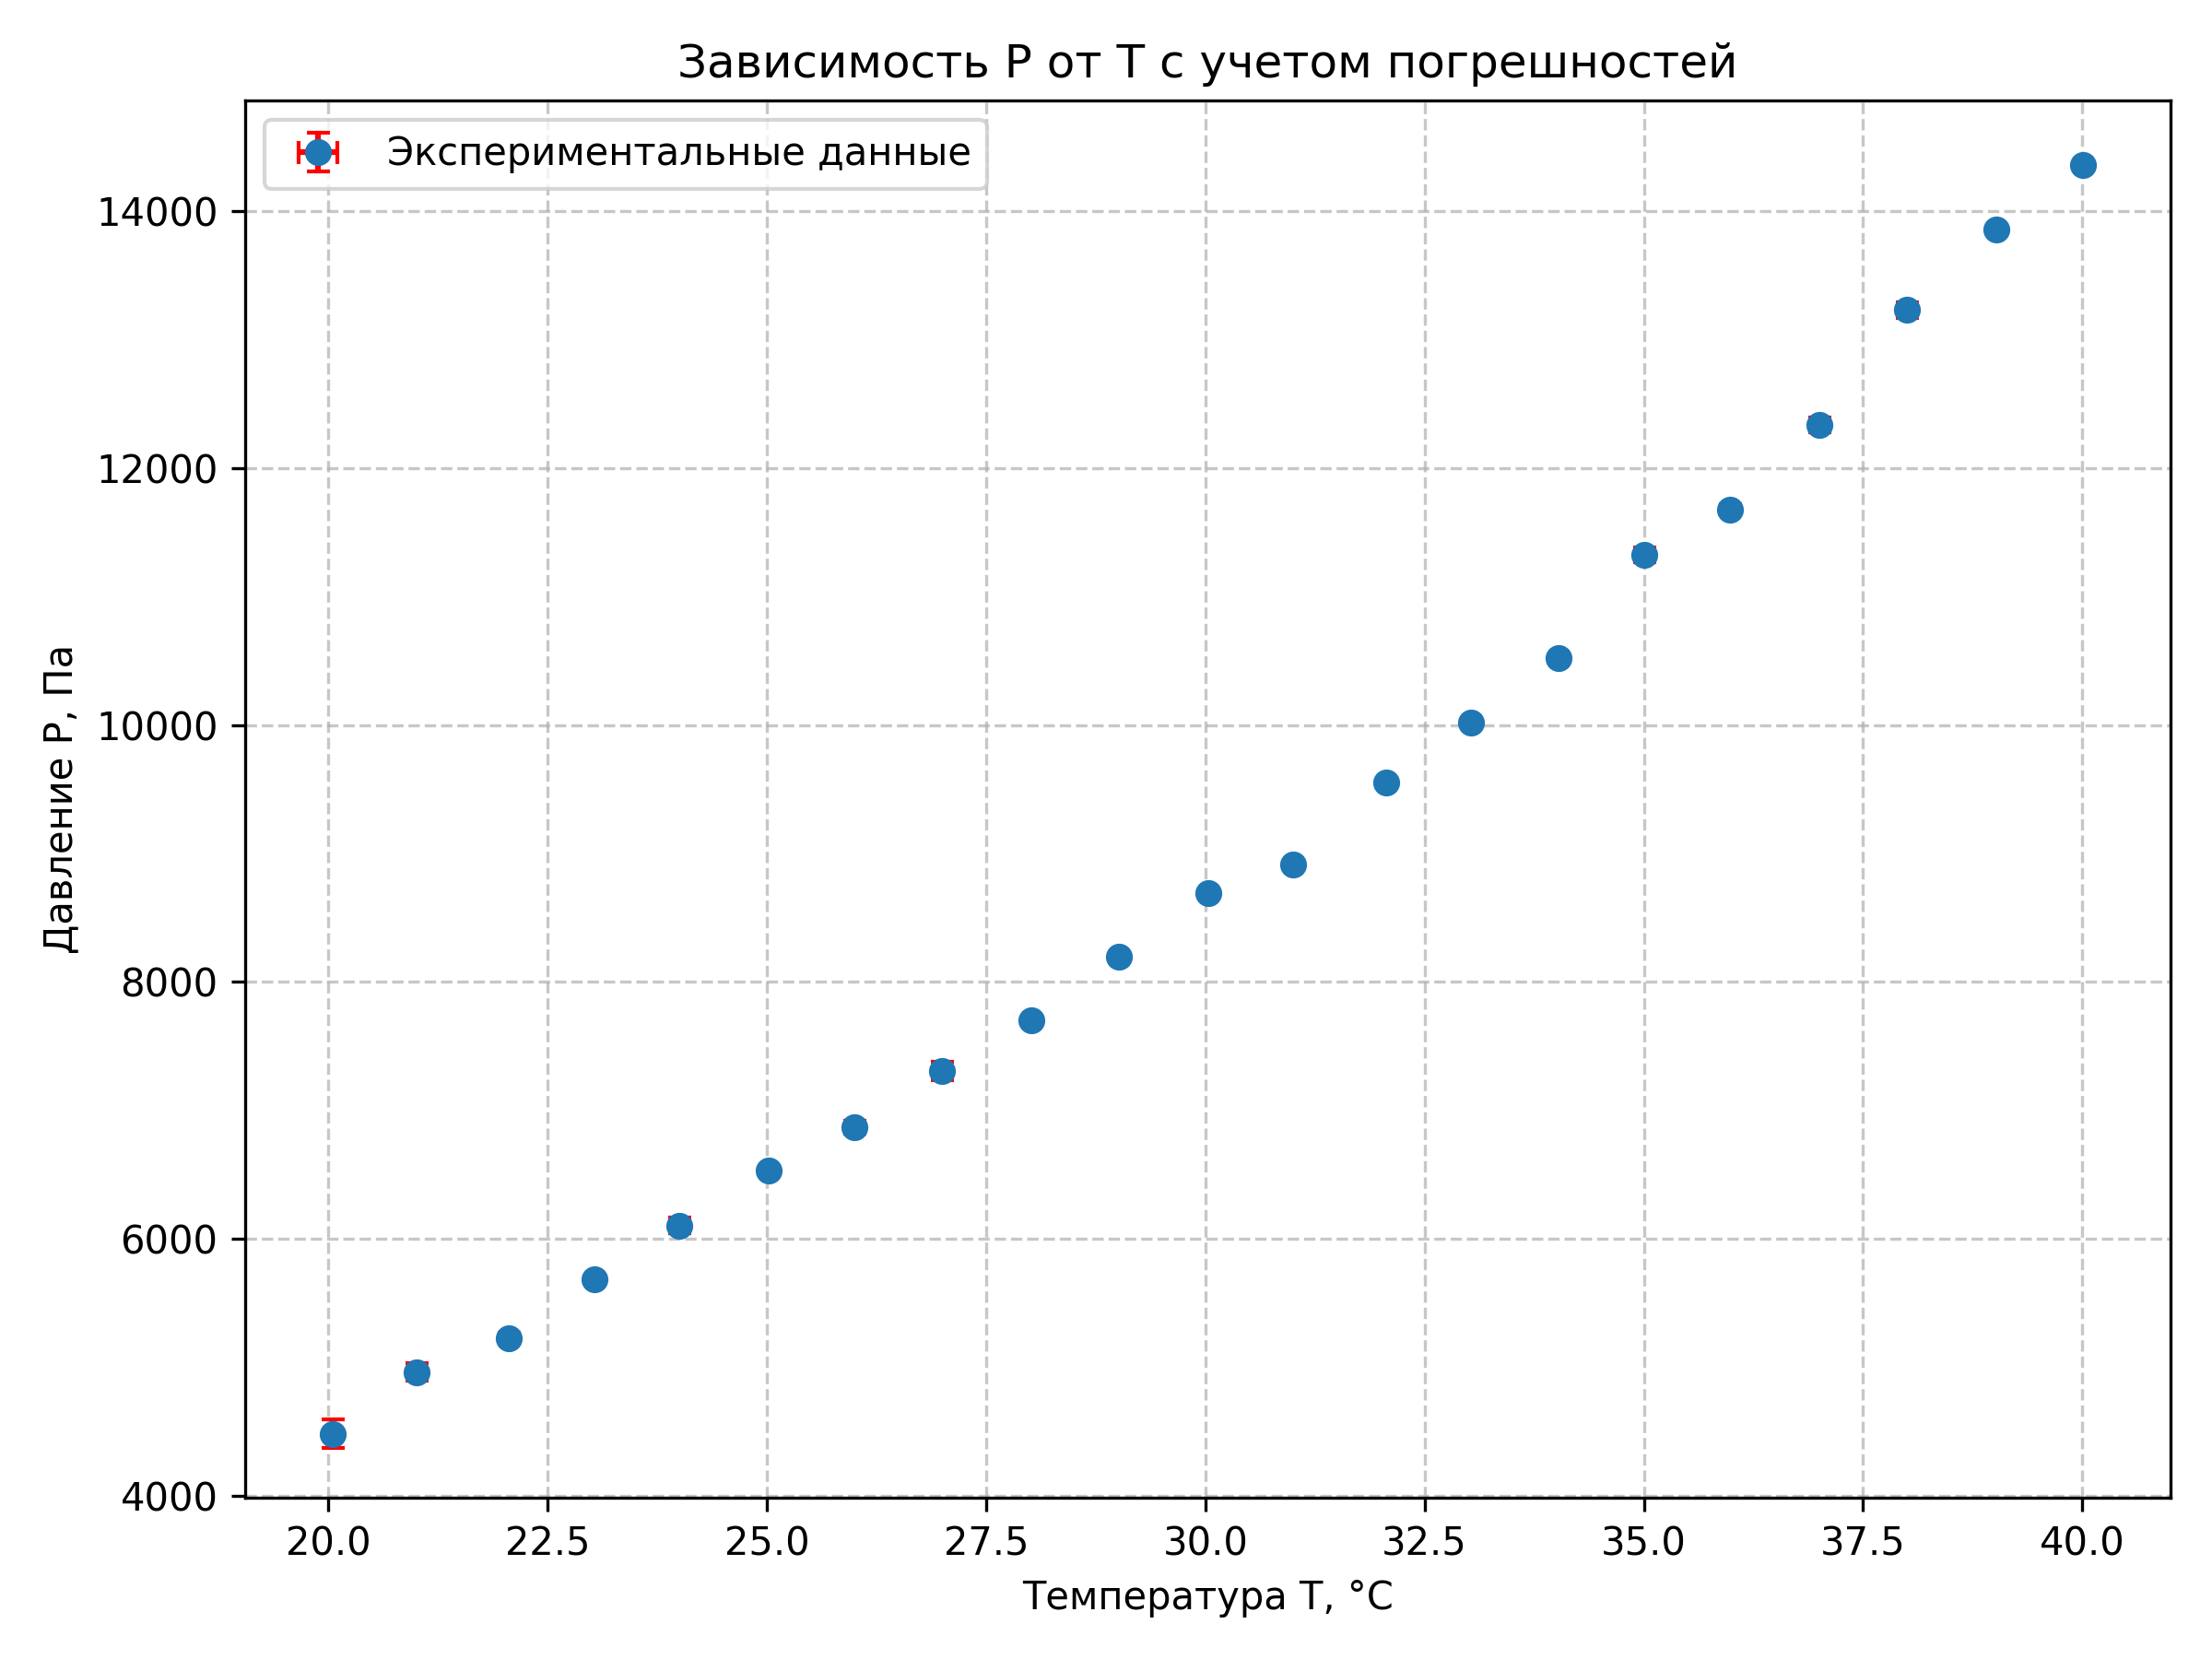
\includegraphics[scale = 0.75]{graph1.png}
    \caption{График зависимости $P(T)$}
    \label{fig:graph1}
  \end{figure}

  \begin{figure}
    \centering
    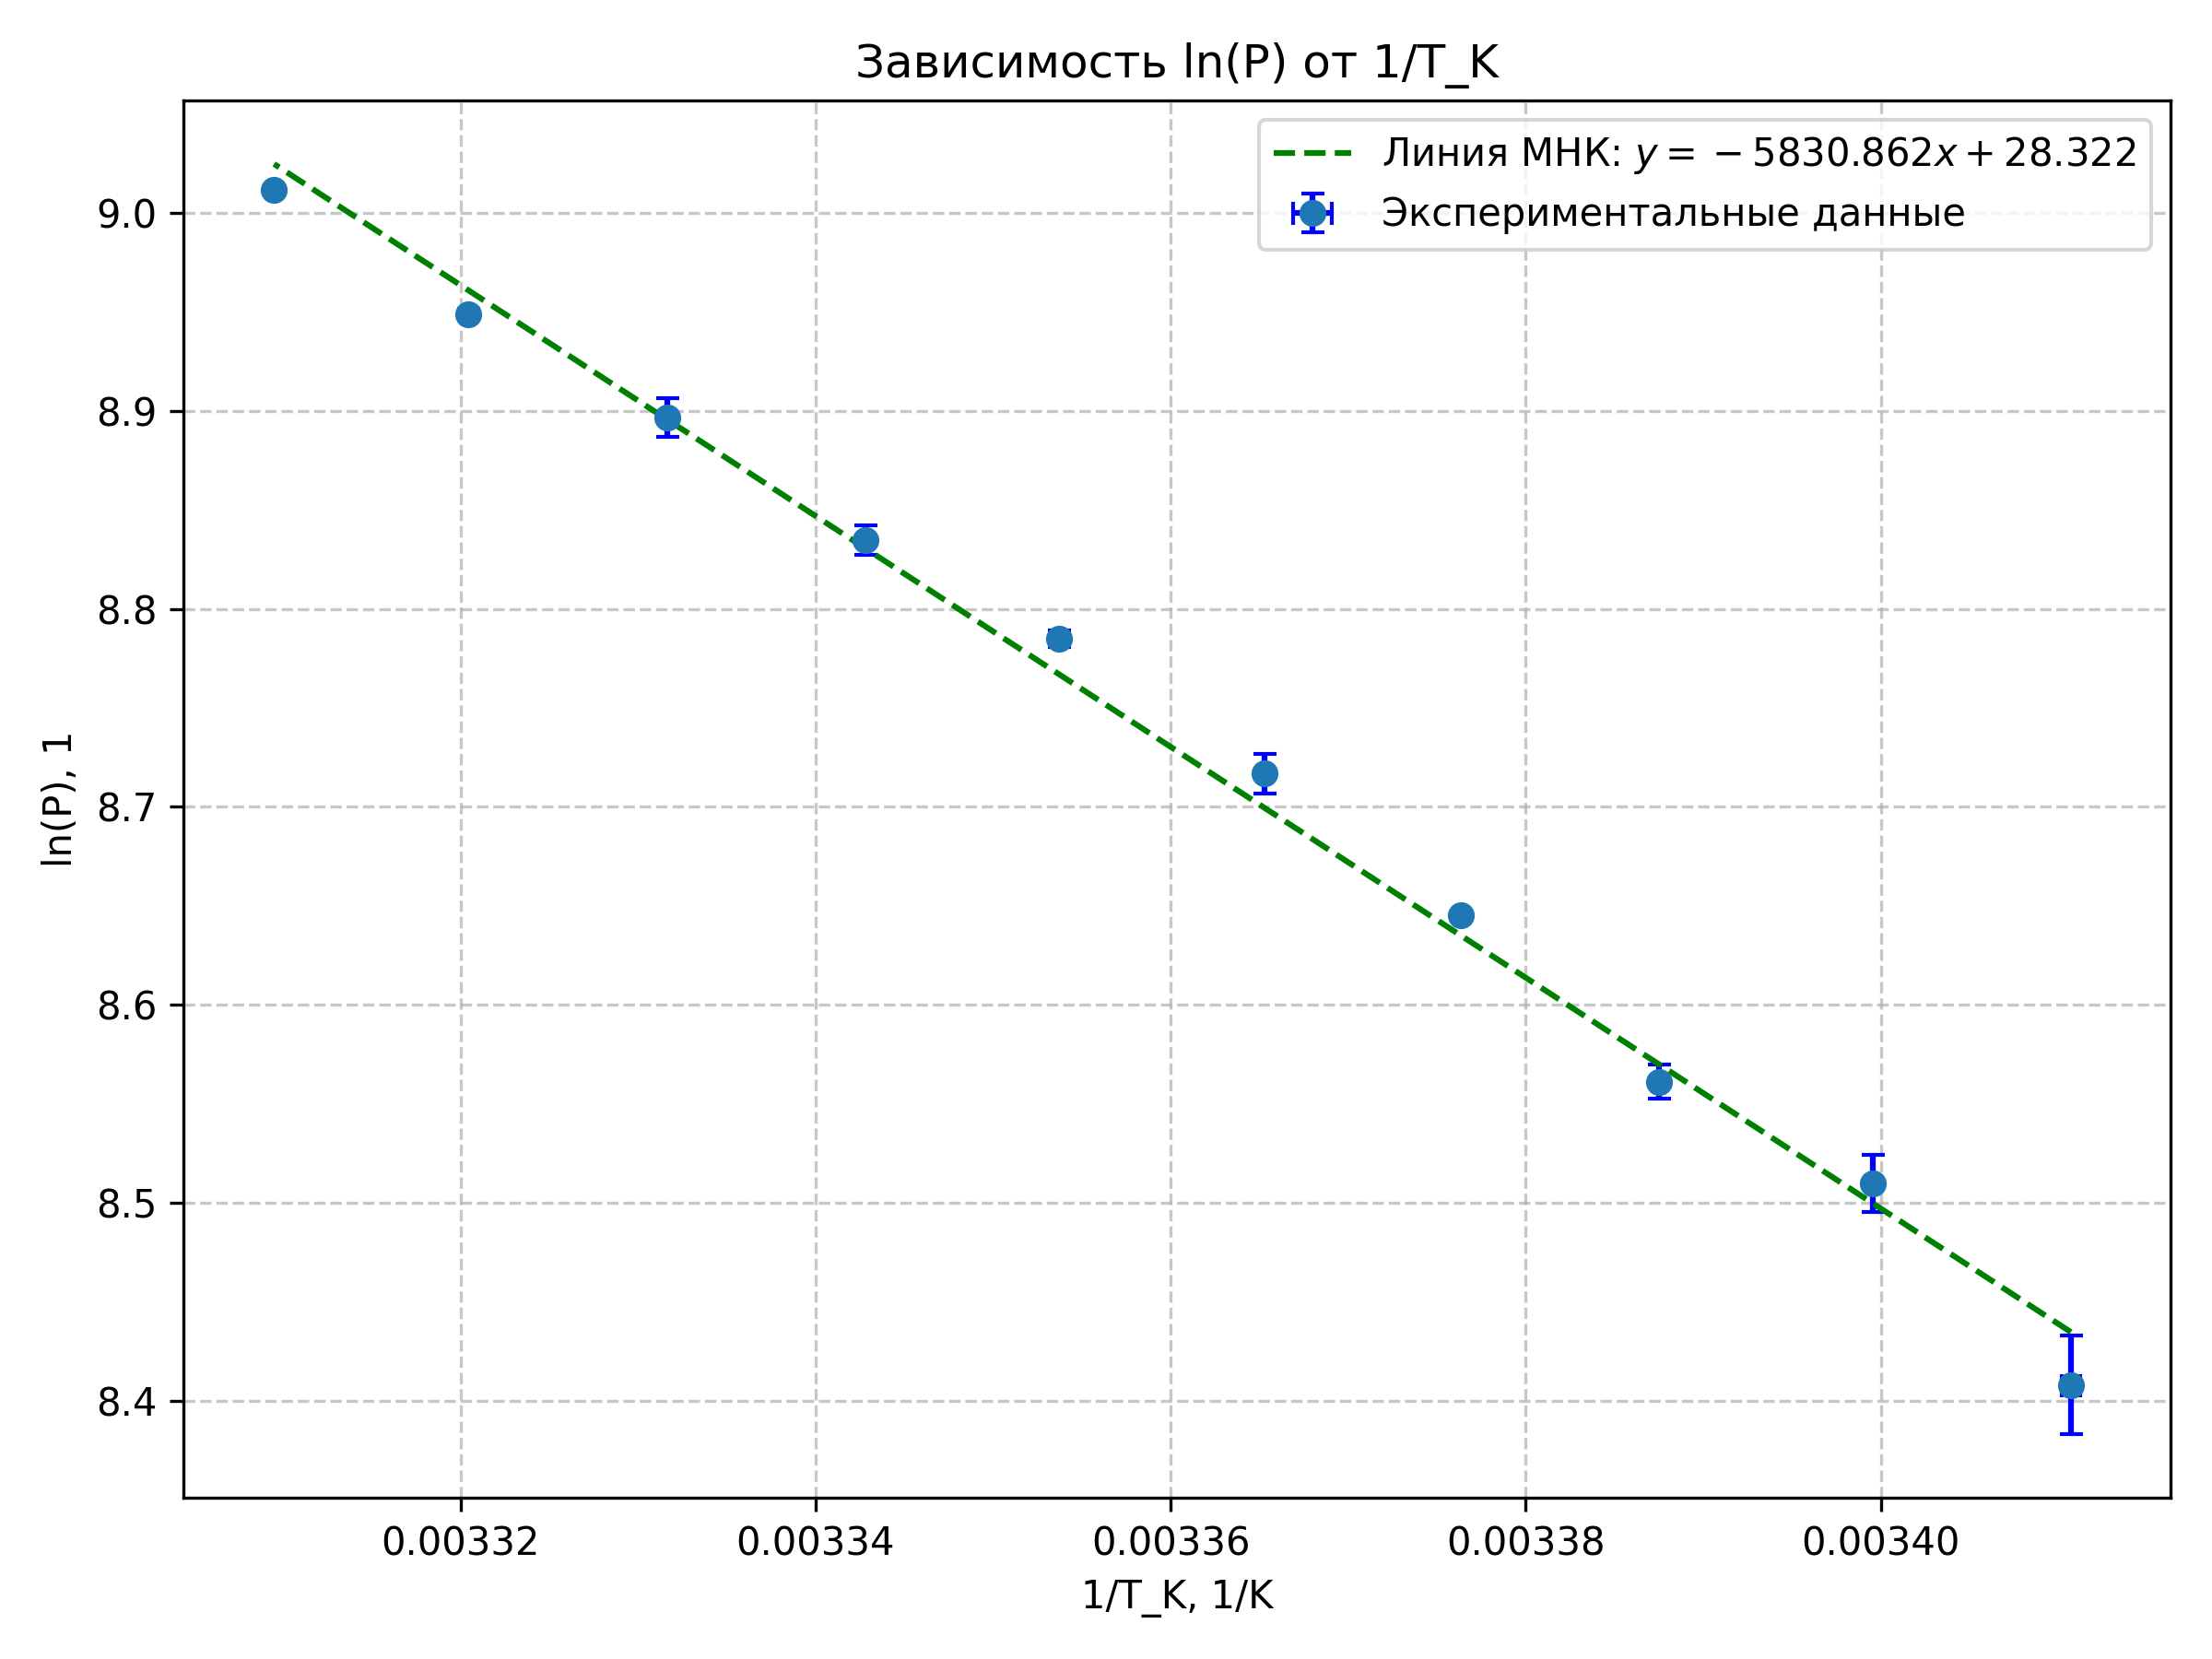
\includegraphics[scale = 0.75]{graph2.png}
    \caption{График зависимости $\mbox{ln}P$ от $1/T_K$}
    \label{fig:graph2}
  \end{figure}

  \item Несмотря на методические рекомендации, по совету нашего преподавателя было принято решение измерения при охлаждении жидкости не проводить.

  \item Вычислим $L$, пользуясь формулой (\ref{L}) и данными, полученными сначала из одного, а потом из другого графика. 
  Сравним результаты, оценим ошибку измерений.

\end{enumerate}
\section*{Обработка результатов измерений}

Найдем молярную теплоемкость жидкости двумя способами.

\subsection*{Метод 1. Линейная зависимость $\mbox{ln}P$ от $1/T_K$}

Найдем угловой коэффициент $k = \frac{d(\mbox{ln}P)}{d(1/T)}$ графика (\ref{fig:graph2}) с помощью метода наименьших квадратов.

\begin{equation}
  \label{k}
  k = \frac{d(\mbox{ln}P)}{d(1/T)} = \frac{\langle \frac{1}{T} \mbox{ln}P \rangle - \langle \frac{1}{T} \rangle \langle \mbox{ln}P \rangle}{\langle \frac{1}{T^2} \rangle - \langle \frac{1}{T} \rangle ^2} = - 5205.51\ K 
\end{equation}

\begin{equation}
  \label{dk}
  dk = \frac{1}{\sqrt{n}} \sqrt{\frac{\langle (\mbox{ln}P)^2 \rangle - \langle \mbox{ln}P \rangle ^2}{\langle \frac{1}{T^2} \rangle - \langle \frac{1}{T} \rangle} - k^2} = 63.83\ K 
\end{equation}

\begin{equation}
  \label{ek}
  \varepsilon_{k_{\text{МНК}}} = \left| \frac{dk}{k} \right| = 0,012
\end{equation}

Учтем погрешность прямых измерений.

\begin{equation}
  \varepsilon_{k_{\text{ИЗМ}}}= \varepsilon ({d(\mbox{ln}P)}) + \varepsilon({d(1/T)}) = \frac{dP}{P} + \frac{dT}{T_K^2} = 0.007
\end{equation}

Получается:
\begin{equation}
  \varepsilon_k = \varepsilon_{k_{\text{МНК}}} + \varepsilon_{k_{\text{ИЗМ}}} = 0.019
\end{equation}

Вычислим молярную теплоту испарения вещества $L$, пользуясь формулой (\ref{L}). Возьмем $R = (8.3145 \pm 0.0001)$, чтобы $\varepsilon_R \ll \varepsilon_k$.

\begin{equation}
  L = -kR = 43 279\ \frac{\mbox{Дж}}{\mbox{моль}}
\end{equation}

Пользуясь $\varepsilon_k =  \varepsilon_L$:
\begin{equation}
  dL =  |\varepsilon_L L| = 832\ \frac{\mbox{Дж}}{\mbox{моль}}
\end{equation} 

Итак,

\begin{equation}
  L = (4.33 \pm 0.08) \cdot 10^{4}\ \frac{\mbox{Дж}}{\mbox{моль}} \qquad (1,9\%) 
\end{equation}


\subsection*{Метод 2. Зависимость $P$ от $T$}

Из графика (\ref{fig:graph1}) заметно, что зависимость не линейная. 

Вычислим значения теплоты испарения $L$ в каждой точке графика, за исключением крайних. 
Для каждой такой точки построим касательную, приблизив кривую зависимости $P(T)$ параболой, 
построенной по этой точке и двум ближайшим к ней (т.е. соседним). 

Заметим, что значения температуры в точках графика меняется на одну и ту же величину 
с каждым следующим измерением, благодаря чему соответствующая секущая — прямая, проходящая через соседние к данной точки 
графика, — параллельна касательной. 

Найдем угловой коэффициент секущей и его погрешность:

\begin{equation}
  \label{sec}
  k_i = \frac{dP}{dT} = \frac{P_{i + 1} - P_{i - 1}}{T_{i + 1} - T_{i - 1}}
\end{equation}

\begin{equation}
  \label{eps_k_i}
  \varepsilon_{k_i} = \varepsilon_{P_{i + 1}} + \varepsilon_{P_{i - 1}} + 2\varepsilon_{T_{i + 1}} + 2\varepsilon_{T_{i - 1}}
\end{equation}

Для каждой точки подставим значение углового коэффициента секущей в уравнение (\ref{L}) и вычислим теплоту испарения $L$ и её погрешность:

\begin{equation}
  L_i = \frac{RT_i^2}{P_i}\left(\frac{dP}{dT}\right)_i = \frac{RT_i^2}{P_i}k_i
\end{equation}

\begin{equation}
  \label{eps_L_i}
  \varepsilon_{L_i} = \varepsilon_{k_i} + 2\varepsilon_{T_i} + \varepsilon_{P_i} 
\end{equation}

\begin{equation}
  dL_i = \varepsilon_{L_i} L_i
\end{equation}

Полученные значения занесем в таблицу (\ref{tab:k_i_L}).

\begin{table}[h]
  \centering
  \begin{tabular}{|c|c|c|c|c|}
    \hline
    $k_i,\ \frac{\text{Па}}{\text{К}}$ & $L_i,\ \frac{\text{Дж}}{\text{моль}}$ & $dL,\ \frac{\text{Дж}}{\text{моль}}$ & $T,\ K$ \\
    \hline
    369.05 & 53493 & 2854 & 294.16 \\
    355.34 & 49277 & 1460 & 295.21 \\
    452.27 & 58045 & 1457 & 296.18 \\
    426.66 & 51312 & 1047 & 297.15 \\
    382.01 & 43218 & 1123 & 298.18 \\
    391.35 & 42394 & 1083 & 299.15 \\
    412.28 & 42262 & 1011 & 300.15 \\
    442.51 & 43342 & 802  & 301.17 \\
    491.29 & 45500 & 422  & 302.16 \\
    361.57 & 31801 & 286  & 303.18 \\
    425.44 & 36694 & 354  & 304.16 \\
    543.77 & 44086 & 503  & 305.21 \\
    493.48 & 38391 & 414  & 306.18 \\
    662.91 & 49413 & 620  & 307.18 \\
    590.99 & 41189 & 545  & 308.16 \\
    504.76 & 34335 & 532  & 309.14 \\
    772.62 & 50085 & 748  & 310.16 \\
    757.57 & 46079 & 587  & 311.15 \\
    562.87 & 32902 & 315  & 312.16 \\
    \hline
  \end{tabular}
    \caption{Значения $k_i$, $L_i$ и их погрешностей}
    \label{tab:k_i_L}
\end{table}

Найдем среднее значение теплоты испарения на данном диапазоне и ее случайную погрешность.

\begin{equation}
  \langle L \rangle = 43885,11\ \frac{\mbox{Дж}}{\mbox{моль}} 
\end{equation}

\begin{equation}
  \varepsilon_{{\langle L \rangle}_{\text{СР}}} = \frac{d\langle L \rangle}{\langle L \rangle} = 0.021
\end{equation}

Учтем погрешность прямых измерений. Мы уже находили ее в первом методе, поэтому воспользуемся полученным значением. Однако в этом случае она умножается на количество $N = 19$ рассчитанных точек.

\begin{equation}
  N \cdot \varepsilon_{{\langle L \rangle}_{\text{ИЗМ}}} = 19 \cdot 0.007 = 0.132
\end{equation}

Таким образом,

\begin{equation}
  \varepsilon_{{\langle L \rangle}} = \varepsilon_{{\langle L \rangle}_{\text{СР}}} + \varepsilon_{{\langle L \rangle}_{\text{ИЗМ}}} = 0.132 + 0.021 = 0.153
\end{equation}
\begin{equation}
  d\langle L \rangle = \varepsilon_{\langle L \rangle} \langle L \rangle = 6732,64\ \frac{\mbox{Дж}}{\mbox{моль}} 
\end{equation}
\begin{equation}
  \langle L \rangle = (4.4 \pm 0.7) \cdot 10^{4}\ \ \frac{\mbox{Дж}}{\mbox{моль}} \qquad (15\%)
\end{equation}

Для визуализации полученных данных построим график $L$ от $T$ (\ref{fig:graph3}).

\begin{figure}[h]
  \centering
  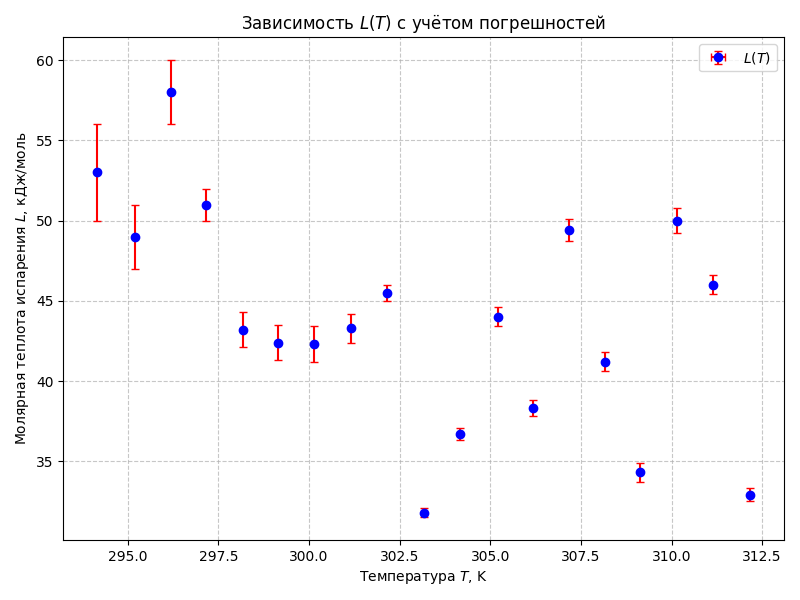
\includegraphics[scale = 0.75]{graph3.png}
  \caption{График зависимости $L(T)$}
  \label{fig:graph3}
\end{figure}

Значения сильно разбросаны, но можно заметить уменьшение значения молярной теплоты испарения $L$ с ростом температуры $T$. 
Это позволяет предположить зависимость величины теплоты испарения от температуры.

\section*{Вывод}

Все цели работы были достигнуты. 

\begin{enumerate}
  \item Значения давление насыщенного пара $P$ при разных температурах $T$ представлены в таблице (\ref{tab:lnP_1T}). 
  \item По полученным данным вычислена величина теплоты испарения с помощью уравнения Клайперона-Клаузиуса (\ref{Klap}) 
  двумя способами: из линейного коэффициента зависимости $\mbox{ln}P$ от $1/T_K$ и с помощью поиска касательной к графику $P(T)$. 
  
  Согласно первому методу:
  \begin{equation}
    L = (4.33 \pm 0.08) \cdot 10^{4}\ \frac{\mbox{Дж}}{\mbox{моль}} \qquad (2\%) 
  \end{equation}

  Согласно второму методу:
  
  \begin{equation}
    L = (4.4 \pm 0.7) \cdot 10^{4}\ \ \frac{\mbox{Дж}}{\mbox{моль}} \qquad (15\%)
  \end{equation}
\end{enumerate}

Метод определения значения молярной теплоты испарения $L$ с использованием углового коэффициента зависимости $\mbox{ln}P$ от $1/T_K$ позволяет получить более точное значение $L$. 

Второй метод менее точен ($15\%$), однако позволяет измерить значения  $L$ для каждого значения температуры, кроме крайних, проследить зависимость $L(T)$ и сделать вывод о её характере: 
предположить, что теплота испарения $L$ уменьшается с ростом температуры $T$ для этой жидкости.

\end{document}
